\chapter{Formulas prescribe Induction}\label{chp:grammar}

% \begin{figure}[!h]
\begin{tikzpicture}
    \fill[black] (0,0) rectangle (5.25in,-7in);

    %
    \node at (2.75cm,-2.75cm) {
        \includegraphics[width=5cm,trim={60 50 50 60 },clip]{induction.png}
    };
    \node at (8.5cm,-2.5cm) {
        \includegraphics[width=6cm,trim={0 50 0 0},clip]{induction-2.png}
    };

    %
    \node at (4.5cm,-6.5cm) {
        \includegraphics[width=5cm,trim={0 100 0 0 },clip]{induction-3.png}
    };
    \node at (10cm,-6.5cm) {
        \includegraphics[width=5.5cm,trim={0 80 0 0 },clip]{induction-4.png}
    };

    %
    \node at (2.5cm,-11cm) {
        \includegraphics[width=5cm,trim={0 100 0 0 },clip]{induction-5.png}
    };
    \node at (8cm,-11cm) {
        \includegraphics[width=5.5cm,trim={0 80 0 0 },clip]{induction-6.png}
    };

    %
    \node at (4cm,-15cm) {
        \includegraphics[width=6cm,trim={0 0 0 0 },clip]{induction-7.png}
    };

    \node at (10cm,-15cm) {
        \includegraphics[width=5.5cm,trim={0 80 0 0 },clip]{induction-8.png}
    };
\end{tikzpicture}
% \end{figure}

\newpage
~
\vspace{5in}
% \begin{figure}[!h]
\begin{tikzpicture}
    \fill[black] (0,0) rectangle (3.75in,-3.25in);
    \fill[black] (1.25in,-3in) rectangle (5in,-5.75in);

    %
    \node at (5cm,-4cm) {
        \includegraphics[width=8cm,trim={0 0 0 0},clip]{induction-9.png}
    };
    \node at (8cm,-11cm) {
        \includegraphics[width=8cm,trim={0 0 0 0},clip]{induction-10.png}
    };
\end{tikzpicture}
% \end{figure}


\chapter{Grammar school}

\begin{quote}
``... small number
of symbols and their grammar are enough to capture the huge
variety of equations...''
\end{quote}

The point of a variable is to replace it.  So in the formula 
$x(x+3)^2$ replacing $x$ for $7$ gives us $7(7+3)^2$.  
Yet even in the land of pure algebra where every symbol is variable it is absurd to
replace $+$ for $7$ to get $x(x73)^2$.   There is restraint in the substitution
of algebra built into what makes something an algebraic formula. When we pull 
on this thread we unravel an expansive relationship between free algebras and induction
and their role in computation.
% \medskip

% It is none other than grammar.

Consider how we know what to do when   
calculating $7(7+3)^2$.  For some of us a mnemonic springs to mind
(\emph{Please Excuse My Dear Aunt Sally}) or an acronym (PEMDAS).
These both unwind to tell us: Parenthesis Exponents Multiplication Division Addition Subtraction
in that order. This meandering thought process somehow elucidates how to read a formula. 
It gives the symbols complex structure that 
can be visualized with the following comic strip.
\begin{center}
    \begin{tikzpicture}[yscale=0.65]
        \node (A) at (0,0) {\begin{tikzpicture}[yscale=0.75]
        \node (f) at (0,0) {$7(7+3)^2$};
        \node[below of=f,scale=0.75] {$\times$};
        \node (x1) at (-1,-2) {$7$};
        \node (sqrt1) at (1,-2) {$(7+3)^{2}$}; 
        % \node[below of=sqrt1,scale=0.75] {$\circ$};
        \node (su) at (1.5,-3) {\textasciicircum $2$};
        \node (u) at (1,-4) {$7+3$};
        \node (x2) at (0,-6) {$7$};
        \node[below of=u,scale=0.75] {$+$};
        \node (three) at (2,-6) {$3$};
        % \node (x3) at (0,-8) {$x$};
        % \node (x4) at (2,-8) {$x$};
        % \node[below of=x2,scale=0.75] {$\times$};

        \draw[-] (f) -- (x1);
        \draw[-] (f) -- (sqrt1);
        % \draw[-] (sqrt1) -- (su);
        \draw[-] (sqrt1) -- (u);
        \draw[-] (u) -- (x2);
        \draw[-] (u) -- (three);
        % \draw[-] (x2) -- (x3);
        % \draw[-] (x2) -- (x4);

    \end{tikzpicture}};
    
    \node[right of=A,xshift=3cm] (B) {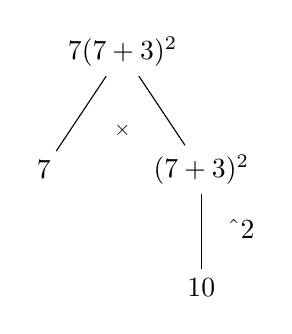
\begin{tikzpicture}[yscale=0.75]
        \node (f) at (0,0) {$7(7+3)^2$};
        \node[below of=f,scale=0.75] {$\times$};
        \node (x1) at (-1,-2) {$7$};
        \node (sqrt1) at (1,-2) {$(7+3)^{2}$}; 
        % \node[below of=sqrt1,scale=0.75] {$\circ$};
        \node (su) at (1.5,-3) {\textasciicircum $2$};
        \node (u) at (1,-4) {$10$};

        \draw[-] (f) -- (x1);
        \draw[-] (f) -- (sqrt1);
        % \draw[-] (sqrt1) -- (su);
        \draw[-] (sqrt1) -- (u);

    \end{tikzpicture}};
    
    \node[right of=B, xshift=3cm] (C) {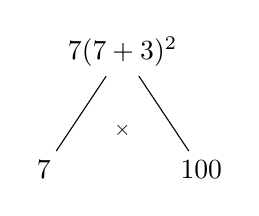
\begin{tikzpicture}[yscale=0.75]
        \node (f) at (0,0) {$7(7+3)^2$};
        \node[below of=f,scale=0.75] {$\times$};
        \node (x1) at (-1,-2) {$7$};
        \node (sqrt1) at (1,-2) {$100$}; 

        \draw[-] (f) -- (x1);
        \draw[-] (f) -- (sqrt1);

    \end{tikzpicture}};
    \node[right of=C,xshift=1cm] {$700$};

    \draw[thick] (A.north east) -- (A.south east);
    \draw[thick] (B.north east) -- (B.south east);
    \draw[thick] (C.north east) -- (C.south east);
\end{tikzpicture}
\end{center}
These step-by-step instructions start at the leaves $7$ and $3$ and join them as $7+3$ (computing $10$),
then the next step is to square (now $100$), then multiply by $7$, we reach $700$.
In hindsight, PEMDAS taught children a complicated form of induction.

\subsection{Induction \& Grammar}
You may have been taught induction through stories of falling 
dominos.  Good.  But what if induction was more like what we just did, climbing?
The domino illustration could bottle up the experience of climbing stairs.  
Now we climb trees and maybe mountains.
Setting up this induction was nothing more than a fragment of text but 
read through the lens of a grammar, e.g.\ PEMDAS, it came into a full form
as steps for recursion.

Parsing grammars in natural language is not always clarifying.  A simplistic
English grammar will often parse into cycles.
\begin{center}
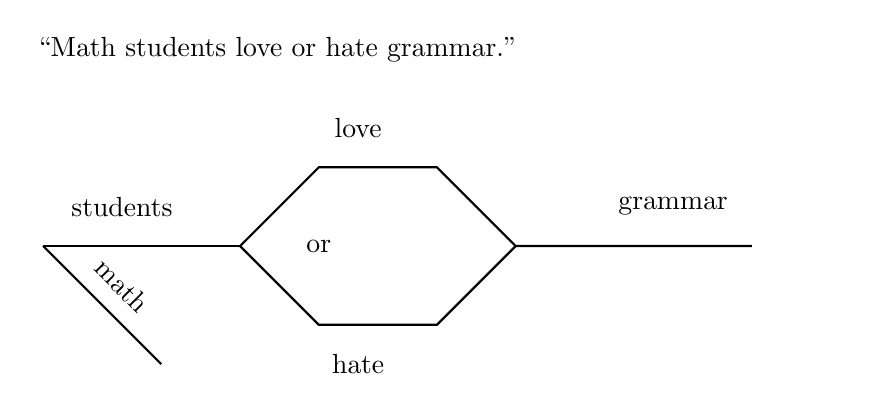
\begin{tikzpicture}
    \node[text width=4in] at (1,2) {``Math students love or hate grammar.''};
    \node at (-3,0) {students};
    \node[rotate=-45] at (-3,-1) {math};
    \node at (-0.5,-0.5) {or};
    \node at (0,1) {love};
    \node at (0,-2) {hate};
    \node at (4,0) {grammar};

    \draw[thick] (-4,-0.5) -- ++(2.5,0);
    \draw[thick] (-4,-0.5) -- ++(1.5,-1.5);
    \draw[thick] (-1.5,-0.5) -- ++(1,1) -- ++(1.5,0) -- ++(1,-1) -- ++(3,0);
    \draw[thick] (-1.5,-0.5) -- ++(1,-1) -- ++(1.5,0) -- ++(1,1);

\end{tikzpicture}
\end{center}
So our inductive climbs may one day need many routes, even go in cycles.
Fortunately, evaluating a formula has a precise algorithm without ambiguity. The
reason is that we had a rooted tree.  Trees have unique paths between any two
vertices. So if we start at the leaves we have a unique direction to reach the
root. 



\index{context-free}
That we got a tree in math formulas means we have a rather boring grammar, 
what Chompsky's \emph{Syntactic Structure} calls
\emph{context-free} grammars.\footnote{
    If an algebraist starts a talk with a story that ``...It was thought  all natural 
    languages were context-free until some obscure dialect in the alps or Africa was found...'', 
    then tune out until they return to equations.  
    Linguist never had such illusions. Even english is not context-free, read  James Higginbotham.} 
Don't be too disheartened.  Virtually every programming language has a 
context-free grammar and programs can communicate a lot of hefty ideas. 

\begin{quote}
    \textbf{Complex inductions can be specified by grammar.}
\end{quote}

\chapter{Natural numbers as grammar}
\index{natural numbers|(}
Math in early history (early childhood) is counting.  Count 
pebbles or beads and give the patterns names
\begin{center}
    $0\defeq$ \underline{\hspace{5mm}}, 
    $1\defeq$ \StrokeOne,
    $2\defeq$ \StrokeTwo,
    $3\defeq$ \StrokeThree,
    $4\defeq$ \StrokeFour,
    $5\defeq$ \StrokeFive,...
\end{center}
One hypothesis for the symbol
``0'' is that it looks like the shape left by removing the last pebble from
a sand table leaving behind no pebbles.

\index{Peano}
It struck Giuseppe Peano in the early 1900's that tallies would be easier to get
right mathematically than digits. With the following two rules Peano introduced
the natural numbers to the formalism of math.
\begin{quote}
    \textit{
    $N_0$ vale ``numero'', et es nomen commune de 0,1,2, etc.\\
    $0$ $\to$  ``zero''\\
    $+$ $\to$ ``plus''.  Si $a$ es numero, $a+$ indica ``numero sequente $a$''.
    }
\end{quote}
% It is fitting that the Italian is in italics.
(See G. Peano \emph{Formulaire de mathematiques.~I-V}, p.27.)
Replacing $+$ with \StrokeOne ~(and equating \StrokeFive$\defeq$\StrokeFour~\StrokeOne),
Peano's model of numbers is simply the grammar of tallies.

Today notation has evolved.  These numbers are now almost always designated as
\emph{natural numbers} and denoted $\mathbb{N}$.  Instead of $a+$ we now often
write $S~k$  or $S(k)$ calling it the ``successor'' to the natural number $k$.  
Programming however has held closer to the original with notation like 
\code{i++} and \code{++i}.

\index{tag}\index{token}\index{\code{<Token>}}\index{\code{::=}}\index{Walrus}
We mentioned Peano was merely recording a grammar.  Today we write grammars with
list of rules, called \emph{production rules}.  Some rules are to specify what
makes up the alphabet of symbols in our grammar.  For Peano, $0$ and $S$ are the
complete alphabet.  So we may write either $0$ on its own, or we may pre-pend
the symbol $S$ to any existing natural number.  Each rule is given a name called
a \emph{token} (or \emph{tag}) and denoted \code{<Name>}. Since the Walrus
$\defeq$ is our assignment of variables (more on this later), we use the
``astonished Walrus'' $::=$ as assignment of production rules.   Taken together
the grammar is the following, shown next to the childhood grammar for tallies.
\begin{center}
\begin{minipage}{0.4\textwidth}
\begin{Gcode}[]
<Nat> ::= 0 
<Nat> ::= S <Nat>
\end{Gcode}
\end{minipage}
\hfill
\begin{minipage}{0.45\textwidth}
\begin{Gcode}[]
<Tally> ::=  
<Tally> ::= | <Tally>
\end{Gcode}
\end{minipage}
\end{center}
In the first rule we are told \code{0} is a natural number, denoted
\code{0:Nat}, just as any whitespace can start a tally. We say that the natural
number grammar \emph{accepts} \code{0} because it matched some production rule,
and the Tally grammar accepts whitespace, usually denoted $\epsilon$.  In the
second rule if we encounter an \code{S} it must be followed by an \emph{already
known} natural number.  So \code{S0:Nat} but \code{0S} would not be accepted as
it is not found as a production rule.  Going forward we use $\mathbb{N}$ 
for \code{Nat} and the usual name $0,1\defeq S0, 2\defeq SS0,\ldots$ as is common.
We retain the notation $n:\mathbb{N}$, instead of $n\in \mathbb{N}$, on account 
of the view that we need natural numbers well before we have a notion of Set Theory.

\index{language}
\begin{definition}
    The words (also called strings) of letters accepted by a grammar is called
    the grammar's \emph{language}.
\end{definition}

\begin{example}
The natural numbers are the language of Peano's grammar, that is, the language of tallies.
\end{example}

The significance of the ``already known'' clause of the rules is to prevent ambiguity 
with terms like $n=$\code{SSS....} where the \code{S} continue forever.
For if we remove one \code{S} form this $n$, the string is unchanged (thanks to 
the infinite number of $S$'s).  Since we are engaged in deciding if $n$ is a natural number and its substring 
is $n$, it is not of the form \code{S k} for \code{k:Nat}.  Hence the grammar 
rejects such an $n$.  Grammar's like these are called \emph{primitive recursive}
meaning that the recursion can only depend backwards 
in history.

\begin{definition}
    A production rule that appears more than once is called \emph{inductive}.
\end{definition}

An accepted short hand for inductive productions rules is to name it once 
and separate the cases by $\mid$, for instance,
\begin{center}
\code{<Nat>::= 0 | S <Nat>} \\
\begin{Gcode}[]
<Nat> ::= 0 
        | S <Nat>
\end{Gcode}
\end{center}
Because of this notation for inductive types I will hence forth limit my use of tallies
to avoid confusion, but I stress that a simplicity often emerges from thinking 
of tallies instead of successors.
    

\begin{remark}{}
    Some argue that $0$ does not ``belong in'' $\mathbb{N}$ because 
    we begin counting at $1$.  Others argue that Peano's postulates
    clarify that $0$ is a natural number and begin counting from there.\\

    Both perspectives miss the point.  Peano is telling us that $\mathbb{N}$
    is not a set of numbers at all.  Instead it is two operators:
    \begin{itemize}
        \item $0$ clears the slate, preparing for a new count.
        \item $S$ successor advances the count.
    \end{itemize}
    So indeed $0$ is required at the start \emph{and} the first count will be $1$.
    The set of numbers created is immaterial.  Its the operations we need for counting.
\end{remark}

\section{Drawings of grammar}
For each accepted word we can associate a graph where the nodes are the
production rule used at that stage to accept the fragment of the string, and
edges are any data needed by that rule to accept the substring.  This is called
the \emph{parse graph}.  In our cases they will always be trees so they are
often called \emph{parse trees}\index{parse tree} but you may also hear them
called \emph{abstract syntax trees} or ``ASTs''.\index{AST}\index{abstract
syntax tree}  In this example $0$ depends on nothing but $S$ depends on an
existing symbol.  Here are the first three parse trees in boxes.
\begin{center}
    \begin{tikzpicture}
    
    \node[draw] (A) at (0,0) {\begin{tikzpicture}
        \node (0) at (0,0) {0};
    \end{tikzpicture}};

    \node[draw] (B) at (3,0) {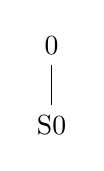
\begin{tikzpicture}
        \node (0) at (0,0) {0};
        \node (S0) at (0,-1) {S0};
        \draw[-] (0) -- (S0);
    \end{tikzpicture}};

    \node[draw] (C) at (6,0) {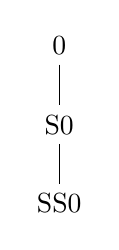
\begin{tikzpicture}
        \node (0) at (0,0) {0};
        \node (S0) at (0,-1) {S0};
        \node (SS0) at (0,-2) {SS0};
        \draw[-] (0) -- (S0);
        \draw[-] (S0) -- (SS0);
    \end{tikzpicture}};
    
    \draw[->] (A) edge["S"] (B);
    \draw[->] (B) edge["S"] (C);
    \draw[dashed,->] (C) edge["S"] (9,0);
\end{tikzpicture}
\end{center}
Between these boxes we have a different graph, the graph that 
plots how one production rule evolves an existing string to another.
This outside graph we call the \emph{word graph}.\index{word graph}  We often condense 
the parse trees to a string to draw the word graph compactly.
\begin{center}
    \begin{tikzpicture}
        \node (0) at (0,0) {0};
        \node (1) at (3,0) {S0};
        \node (2) at (6,0) {SS0};
        \coordinate (3) at (9,0);
        \draw[thick,->] (0) edge["S"] (1);
        \draw[thick,->] (1) edge["S"] (2);
        \draw[dashed,thick,->] (2) edge["S"] (3);
    \end{tikzpicture}
\end{center}

\section{Realizing grammar}

We do well to acknowledge inductive types of data as basic programs. Computers
understand this much. Listing~\ref{lst:peano} shows two programs you could run
today that implement Peano's idea. There are of course many differences.
Visibly, the left-hand side favors mathematically minded symbolic notation and
economizes even on parentheses in the spirit of ``$\sin x$'' notation. Meanwhile
the right-hand side favors a verbose imitation of natural language and prefers
the $\sin(x)$ notation.  Set the differences aside.

\begin{lstfloat}
\begin{center}
\begin{minipage}{0.37\textwidth}
\begin{Fcode}[]
data Nat = Z 
    | S (k:Nat)

zero = Z
two = S (S zero)
\end{Fcode}
\end{minipage}
\hfill
\begin{minipage}{0.62\textwidth}
\begin{Pcode}[language=Sava]
class Nat
  case Zero() extends Nat
  case Next(k:Nat) extends Nat
sealed  // no more cases
zero = new Zero()
two = new Next(new Next(zero))
\end{Pcode}
\end{minipage}
\end{center}
\caption{Peano's natural numbers programmed in two different programming languages.}
\label{lst:peano}
\end{lstfloat}
    

Even without a deep understanding of these programs, one can make out the
contours of Paeno's definitions.  Both use a mix of keywords (in blue) to tell
our system to prepare a new type (or class) of data that will be called
\code{Nat}.  Then they instruct the system to accept exactly two ways to make
such data. It may be some initial state, \code{Z}, respectively \code{Zero},
that depends on nothing; otherwise, we must give data \code{k} of type
\code{Nat}, denoted \code{k:Nat}, which will then produce new data \code{S k},
respectively \code{Next(k)}.  In many systems the keyword \code{new} is 
used to help clue the reader into the fact that this is some data being now 
created.  It helps remind us that numbers do not  exists on their own, 
we have to expend resources (energy \& storage) to create them. 


\section{Eliminating grammar}
    
Now that we have created numbers we shall want to use them.
An obvious use of numbers in counting is to make the process 
modular and parallel.  For example we can have two separate counts 
later combined by addition.
\begin{center}
    \begin{tabular}{c|ccccc}
    ``add'' & \StrokeOne & \StrokeTwo & \StrokeThree & \StrokeFour & \StrokeFive\\
    \hline 
    \StrokeOne & \StrokeTwo & \StrokeThree & \StrokeFour & \StrokeFive & \StrokeOne \StrokeFive\\
    \StrokeTwo & \StrokeThree & \StrokeFour & \StrokeFive & \StrokeOne \StrokeFive & \StrokeTwo \StrokeFive\\
    \StrokeThree & \StrokeFour & \StrokeFive & \StrokeOne \StrokeFive & \StrokeTwo \StrokeFive & \StrokeThree \StrokeFive \\
    \StrokeFour & \StrokeFive & \StrokeOne \StrokeFive & \StrokeTwo \StrokeFive & \StrokeThree \StrokeFive & \StrokeFour \StrokeFive\\
    \StrokeFive & \StrokeOne \StrokeFive & \StrokeTwo \StrokeFive & \StrokeThree \StrokeFive & \StrokeFour \StrokeFive & \StrokeFive \StrokeFive\\
    \end{tabular}
    \hspace{1cm}
    \begin{tabular}{|c|cccccc|}
        \hline 
        + & 0 & 1 & 2 & 3 & 4 & 5\\
        \hline 
        0 & 0 & 1 & 2 & 3 & 4 & 5 \\
        1 & 1 & 2 & 3 & 4 & 5 & 6\\
        2 & 2 & 3 & 4 & 5 & 6 & 7\\
        3 & 3 & 4 & 5 & 6 & 7 & 8\\
        4 & 4 & 5 & 6 & 7 & 8 & 9\\
        5 & 5 & 6 & 7 & 8 & 9 & 10\\
    \hline
    \end{tabular}
\end{center}
Beyond a table we need some formulas.  If we have two groups $m$ and $n$ and each is either nothing 
or a successor to something else, then that leaves us with just four cases 
to consider.
\begin{align*}
    \begin{array}{|c|cc|}
        \hline 
        + & 0 & S(k)\\
        \hline 
        0 & 0 & S(k) \\
        S(\ell) & S(\ell) & S(S(\ell+k))\\
        \hline
    \end{array}
\end{align*}
As the first column does not change $m$ we can simplify this down to 2 cases.
\begin{align*}
    m+n \defeq \begin{cases} m & n=0\\ S(m+k) & n=S(k)\end{cases}
\end{align*}
Lets see this out one some examples, recalling that $1=S0$, $2=S1$, $3=S2$ and so on.
\begin{align*}
    3+2 & = S(3+1)= SS(3+0) = SS3=5.\\
    7+3 & = S(7+2) = SS(7+1) = SSS(7+0)=SSS7=10.
\end{align*}
Notice something about this process is consuming, that is ``eliminating'',
our number $n$ in the sum $m+n$.  

This process gives immediate significance to computation.
To use an inductive type in a program we simply run through the cases.
Programming languages allow for case-by-case analysis in numerous ways 
but most today offer some form of \emph{pattern matching} which is 
where we list the types of production rules and then attach the outcome 
for each.
\begin{lstfloat}
\begin{center}
\begin{minipage}{0.4\textwidth}
\begin{Fcode}[]
+:Nat->Nat->Nat
+ m  0    = m
+ m (S k) = + m k
\end{Fcode}
\end{minipage}
\hfill
\begin{minipage}{0.59\textwidth}
\begin{Pcode}[]
def add(m,n:Nat):Nat =
  match n with 
    Zero() => m
    Next(k)=> Next(add(m,k))
\end{Pcode}
\end{minipage}
\end{center}
\caption{Peano's addition of natural numbers programmed in two different languages.}
\label{lst:peano}
\end{lstfloat}


So in a sense our grammar's role is to guard that data given fits 
a pattern.  Once that has been accepted, when we encounter data 
of this grammar's type we can use that pattern to define functions 
that consume that data.  Historically this is known as \emph{eliminiation}
on account that it may eliminate the data given in the process of 
creating new data as output.

\subsection{Introducing strings}


\subsection{A closer look}
Perhaps the most convincing way to see that we are creating 
data is to run this process all the way down to what a machine 
must do and witness that somewhere the computer must somewhere 
as for storage space.  We will do this 
in stages as the bottom is a mighty long fall.

A first step might be to convert the cases into a sequence 
of two functions which both make appropriate changes to 
some internal value.  This might look like this:
\begin{center}
\begin{lstlisting}[language=Java]
class NaturalNumber {
    int value // Internal computer storage
    Zero() {value=0} // zero out the memory
    Next(k:NaturalNumber){value=k+1}
}
z = new Zero()  // make a 0
two = new Next(new Next(z)) // make a 2
\end{lstlisting}
\end{center}

Grouping this under a single data type `NaturalNumber'
is mostly just for us not to get confused.  When we 
zoom in closer we find that the computer splits 
this apart, making the storage space separate from the 
functions that use it.  Here is a lower level take
and a realization that indeed both introductions (constructors)
need to ask for some storage, they do not really know 
how much, the computer calculates that for them.
\begin{center}
\begin{lstlisting}[language=C]
struct Nat { int length, uint8[] digits }
Nat NaturalNumber_Zero() { 
    memory = malloc(Nat) // allocate memory
    memory.length = 1
    memory.value[0] = 0
    return memory 
}
Nat NaturalNumber_Next(k:Nat) {
    memory = malloc(Nat) // allocate memory
    if k.digits[k.length-1] != 0 then
        memory.length = length +1
    
    memory.digits = k.digits +1
    return memory 
}
\end{lstlisting}
\end{center}

If we zoom in even further we see this `malloc' command eventually 
translate into asking for actual memory in the computer.  Here is a
simplified take that assumes the length is fixed at 9 bytes, that is 
the maximum value reached is $2^{128}$, it would take all the computers 
in the world to tally from $0$ to $2^{128}$ in your lifetime so 
this is a safe limit.
\begin{center}
\begin{lstlisting}[language={ [x86masm]Assembler}]
%macro NaturalNumber_Zero 0
    mov param1, 0x0009      ; move 4 into first parameter
    call malloc            ; storage of size param1 (=9)
    mov store, 0x0000      ; mov 0 into the storage
    ret 

%macro NaturalNumber_Next 1
    int  temp
    mov  temp, param1     ; make a copy of first input
    mov param1, 0x0009      
    call malloc          ; storage of size 9
    mov  store, temp     ; move input to storage
    inc  store           ; increment storage 
    ret 
\end{lstlisting}
\end{center}

As this snippet reveals this program comes to a physical limit 
once we exceed the internal storage capabilities of integers in the
system.  We can fix this but the spirit of the programs above 
is to separate the need to understand the computer deeply and see the 
overall behavior.



If we hold on only to these ideas then we are narrowing what we need 
to know about natural numbers to just some fixed rules, so far the rules 
on how to create them.  So let us say that the symbol $\mathbb{N}$ represents 
all the rules that apply to natural numbers and that writing $0:\mathbb{N}$ or 
$n:\mathbb{N}$ is a way of saying that the symbols $0$ and $n$ obey those rules.
Using $\vdash$ to mean  ``yields'', 
In other words
\begin{description}
    \item[Zero] $\vdash 0: \mathbb{N}$, nothing is need to  yield $0$ as a natural number.
    \item[Successor] $k:\mathbb{N}\vdash S(k):\mathbb{N}$, every natural number  $k$ yields 
    another $S(k)$.
\end{description}
We can get back to childhood 
counting by giving names to these Peano numerals
\begin{center}
    $0\defeq 0$,
    $1\defeq S(0)$,
    $2\defeq S(S(0))$,
    $3\defeq S(S(S(0)))$,...
\end{center}
The point is, the successors are not so much a function 
moving around the numbers that we find laying around, it
\emph{makes} numbers.  
If it were not it would not continue forever 
and what would `$\ldots$' and `etc.' mean in your mind?

\subsection{Computational significance.}
Just as we switched Peano's $a+$ to $S(k)$;
it would be no serious issue to have used $a++$, $++a$, or \lstinline{next k}.
Programmers today use a number of alternatives to encode natural 
numbers.  Some languages hold close to mathematical notation 
preferring symbols to have meaning, like the following formula:
\begin{center}
\begin{lstlisting}[language=Hidris]
    data Nat = Z:Nat | S (k:Nat)
\end{lstlisting}
\end{center}
Whatever ``data'' does we can assume it make the computer see what comes 
next as describing a new type of data, `Nat'.  And the symbols 
$Z$ and $S k$ are distributed into cases separated by `|'.

Other languages face business and industry and package data 
verbosely to help communicate the meaning, for example:
\begin{center}
\begin{lstlisting}[language=Sava]
class NaturalNumber
    case Zero extends NaturalNumber
    case Next(k:NaturalNumber) extends NaturalNumber
sealed  // no more cases
\end{lstlisting}
\end{center}
Words like ``data'', ``class'', ``case'' and ``sealed'' are 
called keywords and usually show up in different colors just to make 
sure we notice they have special roles to play in the language.
A successful programming language (PL) will choose keywords 
that have some reasonable ``obvious meaning''.  This means that you 
can learn to read code in most languages by scanning for patterns 
and using keywords as clues to tie the meaning together.  Take 
a moment to see that you see Peano's main idea in both of the above 
code fragments.

\begin{definition}
    In logic rules that explain what produces a symbol are called 
    \emph{introductions}, e.g.\ $\vdash 0:\mathbb{N}$ and 
    $k:\mathbb{N}\vdash S(k):\mathbb{N}$ are introduction rules.
    
    In programming the word \emph{constructor} is often preferred
    as it explains how to construct data of a specified type.        
\end{definition}

\subsection{Reaching new uses.}

The point of basic patterns is to use them in more complex systems
with an understanding of the resulting behavior.  Imagine a string 
of characters in an alphabet \lstinline{Char:=['a','b',...,'z']}.
\begin{lstlisting}[language=Hidris]
data String = Empty | Prepend( head:Char, tail:String) 
\end{lstlisting}
Writing \lstinline{head:Char} or \lstinline{tail:String} 
indicates that head must come from the alphabet we chose 
and tail must be some already produced string, possibly empty.
Some readers might relate to a different dialect of 
programming such as the following
\begin{lstlisting}[language=Sava]
class String
    case Empty extends String
    case Prepend( head:Char, tail:String) extends String
sealed
\end{lstlisting}
The head here caries around what we put in the list and the tail 
is what comes next in the list.  Observe the similarities:
\begin{align}
     2 & \defeq S(S(0)) \tag{$\mathbb{N}$}\\
 \text{\lstinline{"me"}} & \defeq \text{\lstinline{Prepend('m',Prepend('e',Empty))}}
\tag{String}
\end{align}
The left-hand sides are merely notation for what the data really is on the right.
Both the successor and the \lstinline{Prepend} are operators that generate 
new values.  So part of algebra is to generate new data; so, it is no wonder 
that it closely connections to computation.

\subsection*{Exercise}
\begin{enumerate}
    \item Mimic the String data type to make a list of integers (that is 
    switch from the alphabet to integers).

    \index{generics}
    \item Mimic the String data type to make a list of fixed by 
    unknown data of type $A$, call it \lstinline{List[A]}.\footnote{
    Alternatives include \lstinline{List a} and \lstinline{List<A>}. 
    Search for \emph{generics} in your programming language to learn more.
    }

\end{enumerate}
\index{nil}\index{cons}\index{list}
Historically \lstinline{Empty} for lists is called \lstinline{Nil} 
and \lstinline{Prepend} is called \lstinline{Cons}.




% \section{Eliminating grammar}
    
Now that we have created numbers we shall want to use them.
An obvious use of numbers in counting is to make the process 
modular and parallel.  For example we can have two separate counts 
later combined by addition.
\begin{center}
    \begin{tabular}{c|ccccc}
    ``add'' & \StrokeOne & \StrokeTwo & \StrokeThree & \StrokeFour & \StrokeFive\\
    \hline 
    \StrokeOne & \StrokeTwo & \StrokeThree & \StrokeFour & \StrokeFive & \StrokeOne \StrokeFive\\
    \StrokeTwo & \StrokeThree & \StrokeFour & \StrokeFive & \StrokeOne \StrokeFive & \StrokeTwo \StrokeFive\\
    \StrokeThree & \StrokeFour & \StrokeFive & \StrokeOne \StrokeFive & \StrokeTwo \StrokeFive & \StrokeThree \StrokeFive \\
    \StrokeFour & \StrokeFive & \StrokeOne \StrokeFive & \StrokeTwo \StrokeFive & \StrokeThree \StrokeFive & \StrokeFour \StrokeFive\\
    \StrokeFive & \StrokeOne \StrokeFive & \StrokeTwo \StrokeFive & \StrokeThree \StrokeFive & \StrokeFour \StrokeFive & \StrokeFive \StrokeFive\\
    \end{tabular}
    \hspace{1cm}
    \begin{tabular}{|c|cccccc|}
        \hline 
        + & 0 & 1 & 2 & 3 & 4 & 5\\
        \hline 
        0 & 0 & 1 & 2 & 3 & 4 & 5 \\
        1 & 1 & 2 & 3 & 4 & 5 & 6\\
        2 & 2 & 3 & 4 & 5 & 6 & 7\\
        3 & 3 & 4 & 5 & 6 & 7 & 8\\
        4 & 4 & 5 & 6 & 7 & 8 & 9\\
        5 & 5 & 6 & 7 & 8 & 9 & 10\\
    \hline
    \end{tabular}
\end{center}
Beyond a table we need some formulas.  If we have two groups $m$ and $n$ and each is either nothing 
or a successor to something else, then that leaves us with just four cases 
to consider.
\begin{align*}
    \begin{array}{|c|cc|}
        \hline 
        + & 0 & S(k)\\
        \hline 
        0 & 0 & S(k) \\
        S(\ell) & S(\ell) & S(S(\ell+k))\\
        \hline
    \end{array}
\end{align*}
As the first column does not change $m$ we can simplify this down to 2 cases.
\begin{align*}
    m+n \defeq \begin{cases} m & n=0\\ S(m+k) & n=S(k)\end{cases}
\end{align*}
Lets see this out one some examples, recalling that $1=S0$, $2=S1$, $3=S2$ and so on.
\begin{align*}
    3+2 & = S(3+1)= SS(3+0) = SS3=5.\\
    7+3 & = S(7+2) = SS(7+1) = SSS(7+0)=SSS7=10.
\end{align*}
Notice something about this process is consuming, that is ``eliminating'',
our number $n$ in the sum $m+n$.  

This process gives immediate significance to computation.
To use an inductive type in a program we simply run through the cases.
Programming languages allow for case-by-case analysis in numerous ways 
but most today offer some form of \emph{pattern matching} which is 
where we list the types of production rules and then attach the outcome 
for each.
\begin{lstfloat}
\begin{center}
\begin{minipage}{0.4\textwidth}
\begin{Fcode}[]
+:Nat->Nat->Nat
+ m  0    = m
+ m (S k) = + m k
\end{Fcode}
\end{minipage}
\hfill
\begin{minipage}{0.59\textwidth}
\begin{Pcode}[]
def add(m,n:Nat):Nat =
  match n with 
    Zero() => m
    Next(k)=> Next(add(m,k))
\end{Pcode}
\end{minipage}
\end{center}
\caption{Peano's addition of natural numbers programmed in two different languages.}
\label{lst:peano}
\end{lstfloat}


So in a sense our grammar's role is to guard that data given fits 
a pattern.  Once that has been accepted, when we encounter data 
of this grammar's type we can use that pattern to define functions 
that consume that data.  Historically this is known as \emph{eliminiation}
on account that it may eliminate the data given in the process of 
creating new data as output.

Let us now try to eliminate a string.  One example could be to imitate 
our addition of natural numbers, only now we seek an analog to ``add''
strings.  Perhaps concatenation comes to mind.  Using our $[a,b,c]$ 
alphabet ths addition could look like this.
\begin{align*}
    s+t & \defeq \begin{cases}
        t & s=\epsilon\\
        a(w+t) & s= a(w:String)\\
        b(w+t) & s= b(w:String)\\
        c(w+t) & s= c(w:String)\\
    \end{cases}
\end{align*}
Thus,
\begin{align*}
    cab+bab & = c(ab+bab)+c(a(b+bab))=c(a(b(\epsilon+bab)))\\
        & = c(a(b(bab)))=cabbab.
\end{align*}
Once more we can do the same in code by matching the pattern.
Listing~\ref{lst:peano} shows what this might look like for 
strings fixed on the alphabet [a,b,c].  Start to imagine what 
changes you would make to work with other alphabets, and 
eventually interchangeable alphabets.
\begin{lstfloat}
\begin{center}
\begin{Fcode}[]
cat:String_abc->String_abc->String_abc
cat Empty t   = t
cat 'a' tail t = 'a' (cat tail t)
cat 'b' tail t = 'b' (cat tail t)
cat 'c' tail t = 'c' (cat tail t)
\end{Fcode}
\begin{Pcode}[]
def cat(s,t:String_abc):String_abc =
  match s with 
    Empty() => t
    A(tail)=> A(cat(tail,t))
    B(tail)=> B(cat(tail,t))
    C(tail)=> C(cat(tail,t))
\end{Pcode}
\end{center}
\caption{Concatenation of strings over the alphabet [a,b,c] is a variation on 
Peano's addition of natural numbers.}
\label{lst:peano-elim}
\end{lstfloat}
    
% This algorithm remains predictable because of what we assumed about 
% primitive recursion.  That is $m+0$ is defined and if $m+k$ is defined 
% then $m+S(k)\defeq S(m+k)$ is therefore defined.  This is what is 
% known as \emph{recursion}.  It hinges on the fact that the proper 
% \[    P(n) :\equiv m+n \text{ defined}
% \]
% we want is known at step $k$, we write $P(k)$, and so we can 
% use that knowledge to deduce the $m+S(k)$ is defined, in other wards $P(S(k))$ follows.
% \begin{gather*}
%     \begin{array}{rl}
%     P(0)& \\
%     P(k) & \Rightarrow P(k+1)\\
% \hline 
% \forall n:\mathbb{N} & P(n).
%     \end{array}
% \end{gather*}
% This is sometimes known as the principle of induction.  It is more of a program than 
% an assumption of fact.  When we have a $n$ we want to confirm $m+n$ is defined for,
% say $n=SS0$, then we simply apply the rules given repeatedly:
% \[
%     m+SS0=S(m+S0)= SS(m+0)=SS(m)
% \]
% By rule \code{S<Nat>} we get that $SS(m):\mathbb{N}$.  As expected it added two strokes to the 
% tally.   This process of consuming the information given to introduce $n:\mathbb{N}$ is known 
% as \emph{elimination}.   We will see several examples introduction 
% and elimination patterns. 

% If we stand back to observe the entire process, grammars allow us to introduce numbers, 
% such as $2\defeq SS0:\mathbb{N}$.  Then when we have $2:\mathbb{N}$ we can 
% use the data behind its introduction (here two successors and a $0$) as instructions 
% to follow when producing a new outcome, perhaps a new type of data.  This is known 
% as \emph{eliminating} the introduction.  We will see several examples introduction 
% and elimination patterns. 

% \subsection{Type rules}
% We are engaged in forming a type of data, natural numbers.  Some times 
% of data will depend on others, for example tuples $\mathbb{N}^k$ depend on 
% $k$.  So even in the form of types we need to pause and 


% If we break down the 
% steps we first had to give the type a name, 
% If we break this process down here are the summary points.  Note that we use Frege's 
% notation where symbols $p_1,\ldots,p_n$ that lead to symbols $q$ are separated by 
% $\vdash$, so $p_1,\ldots,p_n\vdash q$, which is also often written 
% \begin{align*}
%     \frac{p_1,\ldots,p_n}{q}\qquad 
%     \begin{array}{c}
%         p_1\\
%         \vdots \\
%         p_n\\
%     \hline 
%         q 
%     \end{array}
% \end{align*}
% Note that if nothing is required to lead to $q$ we can write $\vdash q$.
% The symbol $\vdash$ is known formally as \emph{entailment} and while it may 
% appear at first like an implication, it is here being used more in the role of 
% defining rules.
% \begin{gather}
%     \tag{$\form{\mathbb{N}}$}
%     \vdash \mathbb{N}:Type\\
%     \tag{$\intro{\mathbb{N}}$}
%     \vdash 0:\mathbb{N} 
%     \qquad \frac{k:\mathbb{N}}{S(k):\mathbb{N}}\\
%     \tag{$\elim{\mathbb{N}}$}
%     \begin{array}{rl}
%         n &:\mathbb{N}\\
%         P(k) &\vdash P(S(k))\\
%     \hline 
%         P(n)
%     \end{array}
% \end{gather}

% \subsection{Wrapping up errors}
% \begin{center}
% \begin{minipage}{0.35\textwidth}
% \begin{Fcode}
% data Maybe B = 
%     | Just (b:B)  
%     | None 
% \end{Fcode}
% \end{minipage}
% ~
% \begin{minipage}{0.64\textwidth}
% \begin{Pcode}
% class Option[B]
%     case Some(b:B) extends Option[B]
%     case None() extends Option[Any]
% sealed
% def wrap(f:A->B):f:A->Option[B] = 
%     a ->
% \end{Pcode}
% \end{minipage}
% \end{center}
    
\section{Formulas}
It is time to add more sorts of data.  For a change of scene let us look 
at Boolean (true/false) algebra.  Here we have just two ``numerical''
symbols true $\top$,
false $\bot$, but a number of operators: and $\wedge$, or $\vee$, and not $\neg$.
The language might be defined
like this.
\begin{Gcode}[]
<Var>  ::= x | x_<Nat>
<Bool> ::= <Var>
        | $\top$
        | $\bot$
        | $\neg$ <Bool> 
        | <Bool> $\vee$ <Bool> 
        | <Bool> $\wedge$ <Bool>.
\end{Gcode}
Some terms this grammar will except include 
\begin{center}
    $\top \wedge \bot :Bool$, 
    $\neg (x_1\wedge x_2\vee x_3):Bool$, \&
    $\neg(x_1\wedge \neg x):Bool$.
\end{center}
Notice $\top\wedge \bot$ is a Boolean, even though it is not what we might 
consider to be ``true''.   The type of a string is whether it obeys the grammar,
only later do we investigate if this string has any meaning to an applied task.
Notice we the a single letter $x$ is given a different type than $\top,\bot$
hinting at our eventual use of $x$ as a variable.  We even allow our variables 
to take along a natural number so that we can have as many variables as our situation 
should require.  Of course for know this is just a grammar.  It will take using 
the formula to reveal how $x$ behaves like a variable.  At present to be 
a variable only means it is of type ``variable''.



Notice we have clarified in the grammar how 
constants $\top,\bot$ can appear on their own, variables can too.  
Keeping these separate means we can easily swap out our meaning for either.
For example, some boolean systems only allow a fixed number of variables, say 
$x$ and $y$, we would simply adjust to use 
\begin{center}
\code{<Var> ::= x | y}
\end{center}
Also in some applications the constants of truth also have to change.
Intuitionistic logic admits the possibility that that there may be 
things unknowable, so we add to $\top,\bot$ a symbol $?$,
\begin{center}
\begin{Gcode}[]
<Const> ::= $\top$ | $\bot$ | ?
\end{Gcode}
\end{center}
Fuzzy logic considers tolerance and thresholds to accommodate real life uncertainty, 
e.g.\ ``If the bridge is made of 85\% pure steel, then it is 99\% likely to last 50 years.''
Here we may replace \code{<Const>} with a type for intervals [0,1].
In temporal logic, the value of true/false changes with time, so the 
constants have a time parameter.  Modal logic is when truth values 
switch between modes, e.g.\ ``In the day solar power runs the washer; at night 
batteries do.''.  So modes may feature in \code{<Const>}.


\begin{remark}
    There are ways to relate one class of logic to another. 
    For example, G\"odel proved that intuitionistic logic embeds
    in the negative into classical logic.  So you 
    might come away from that saying ``classical logic can do 
    intuitionistic logic.''   As a caution against this perspective note that every integer is 
    a complex number, but we learn a great deal more about integers when we 
    study them with number theory then simply investigating them 
    through complex analysis. 
    % Resist the temptation to toss  
    % aside other logic as special cases of classical logic, less you end up missing 
    % the point.
\end{remark}


Another familiar algebra concerns our customary polynomials.  We will use 
the type \code{<Reals>} describe in a later exercise as the coefficients.
\begin{Gcode}[]
    <Var>  ::= x 
    <UniPolyReals> ::= <Var>
            | <Reals>
            | <UniPolyReals>+<UniPolyReals>
            | (<UniPolyReals>)(<UniPolyReals>)
\end{Gcode}
As is typically  we write $\mathbb{R}[x]$ in place 
of \code{UniPolyReals}.  So this language accepts formulas like these 
\begin{center}
    $1.5+3.4(x)(x):\mathbb{R}[x]$,
    $(x+2)(x-2):\mathbb{R}[x]$, \&
    $12.9:\mathbb{R}[x]$.
\end{center}
This is the minimal requirement for real polynomials.
For example, in this form $x^2+2$ would not be accepted but 
$(x)(x)+2$ would be, and $3x$ would be rejected but $(3)(x)$ would 
be allowed.  We can add extra production rules to accommodate these 
such as \code{<Var>^<Nat>} and \code{<Reals> <Var>} (see exercises).  However, 
these will add more cases to any subsequent elimination of these formulas,
and they introduce ambiguity.  For example, is $x^2$ the same as $(x)(x)$?
It should be but the grammar wont force this.

\begin{remark}
    In point of fact some algebra are not what is known as 
    \emph{power associative} in that $x^n$ is not well-defined 
    on account that we need to know the grouping.  For instance,
    $x(xx)$ need not equal $(xx)x$.

    When a program allows for shortcuts like $3x$ and $x^3$, it is 
    implicitly introducing rules into the algebra which may not be true 
    for all situations.
\end{remark}

Suppose we want to move to polynomials in $x$ and $y$.  Have factored out 
the variables as a separate alphabet we could modify the productions of 
\code{<Var>} leaving the rest unchanged, expect perhaps to rename 
\code{<UniPolyReals>} to \code{PolyReals}.
\begin{Gcode}[]
    <Var>  ::= x | y
    <PolyReals> ::= <Var>
            | <Reals>
            | <PolyReals>+<PolyReals>
            | (<PolyReals>)(<PolyReals>)
\end{Gcode}
We could go one further and alter the use of real numbers to be some other 
kind  of number.  We will call these numbers \code{<Ring>} for now but its 
meaning will be variable until we fixate on evaluation polynomials.
So we now arrive at the general meaning of a polynomial.
\begin{Gcode}[]
    <Poly> ::= <Var>
            | <Ring>
            | <Poly>+<Poly>
            | (<Poly>)(<Poly>)
\end{Gcode}



To formalize the process we have begun we are dealing first in defining types, 
Natural numbers, Strings, \& Booleans.  Now we are engaged in finding common rolls 
amongst the components of these types, e.g.\ constants and variables.
Operators too are set apart in how we use them in the grammar, they are another sort.  They 
need the company of other booleans, or other polynomials.
To designate this division of labor we introduce a new term \emph{sort}.\index{sort}
So we are making a hierarchy to organize our data:
\begin{center}
    terms have types;
    types have sorts.
\end{center}
As with any formalized term there will be examples that blur the boundaries and force 
to revisit the sorting.  Having sorts simply lets us express the difference as we 
find them, it does not in any meaningful way map out a reality.

% \subsection{Eliminating formulas}

% Elimination of a natural number was to work through the tower of successors, 
% but with the introduction of operators we can now depend on many terms.  This 
% is a form of induction with possibly many bases cases.  Our experience with 
% evaluation polynomials offers us a great advantage in guessing how to use these steps.
% We simply draw the parse tree and begin replacing variables with their assigned
% quantities.  We also replace any operator symbols with the algorithm that performs 
% that operation.

% For Boolean algebras the operators may be given by a truth table.
% \begin{align*}
%     \phi \vee \tau \defeq \begin{cases}
%         \top & \phi=\top\\
%         \top & \phi=\bot, \tau=\top\\
%         \bot & \phi=\bot, \tau=\bot
%     \end{cases}
% \end{align*}




\chapter{Context-free grammars}

There is an entire industry of research based on describing what languages 
can come from which grammars and vice-versa.  Its study is today a mixture 
of computer science, algebra, and linguistics.  In those studies one can 
find a rigorous description of grammars and languages along with what 
computational power is needed to  accept a string.  We have already hinted 
at this complication by indicating that we restrict our thoughts to primitive 
recursions so that the process of parsing comes to an end.

\section{Context sensitive grammar}

Now that we have seen a grammar given by production rules we can explain 
in what way context-free grammars are ``context-free'', and how they 
come to parse as trees.  Consider the situation discussing square-roots 
of natural numbers.
\begin{center}
\begin{Gcode}[]
+<Root> ::= + sqrt(<Nat>)
-<Root> ::= - sqrt(<Nat>)
\end{Gcode}
\end{center}
In this case \code{sqrt{2}:<Root>}.  However, we do not know if this 
was meant as the positive or negative root.  That information 
was left to the surrounding context in which the term was parsed.  
This is a very useful situation as often in algebra we do want to 
speak within a context.  Yet because of the ambiguity if we 
introduce a root in this way and then seek to eliminate we 
cannot be certain of many possible paths got us here.

Meanwhile 
to make this context-free grammar we could use 
\begin{center}
\begin{Gcode}[]
<Root> ::= + sqrt(<Nat>)
         | - sqrt(<Nat>)
\end{Gcode}
\end{center}
Now \code{+sqrt(2):<Root>} and \code{-sqrt(2):<Root>} but 
this grammar rejects \code{sqrt(2)}.  The grammar is less forgiving 
but more precise in the content it now holds for us.

\begin{definition}
    A \emph{context-free grammar} is a grammar whose non-constant 
    production rules are defined on the left of the astonished Walrus 
    \code{::=}.
\end{definition}

\begin{remark}
    The symbols \lstinline{::=}, \lstinline{<Token>} and \lstinline{|} are 
    Backus-Naur Form (BNF) notation, which is popular 
    in computer science.  It is actually subject to its own gammar, admittedly 
    basic and fixed in length.  But you can be forgiven for wondering if this is 
    all circular reasoning.  When this occurs, mathematicians like to attach 
    the word \emph{meta}, which means literally ``self-referential''.
    So BNF would be called a \emph{meta-language}. Sometimes self-referential 
    can be turned into paradoxes (Russell's paradox, G\"odel's Incompleteness,
    Turing's Halting problem).  So you may worry.  But I suppose if you 
    didn't believe in language, why would you be reading?\\
\end{remark}

\section{Order of operations.}
There is something still missing.  Try reading $\neg(x_2\wedge y)\vee x_1$.  
Is this meant to negate $(x_2\wedge y)\vee x_1$ 
or is it to negate $(x_2\wedge y)$ and then or that with $x_1$? This grammar 
offers two associated parse trees.
\begin{center}
    \begin{tikzpicture}
        \node at (-3.5,0) {\begin{tikzpicture}
            \node (10) at (0,0) {$\neg(x_2\wedge y)\vee x_1:Bool$};
            \node (0n) at ( 0,-2) {$(x_2\wedge y)\vee x_1:Bool$};
            % \node (0d) at ( 2,-4) {0:Digit};
            \draw[thick] (0n) -- (10);
            % \node[below of=10,scale=0.75] {$\circ$};
            \node at (0.5,-1) {$\neg$};
            % \node[scale=0.75,text width=0.6in] at ( 1.5,-3) {Nat case 1};
        \end{tikzpicture}};
        \node at (3.5,0) {\begin{tikzpicture}
            \node (01) at (0,0) {$\neg(x_2\wedge y)\vee x_1:Bool$};
            \node (1) at (-2,-2) {$\neg(x_2\wedge y):Bool$};
            \node (0n) at ( 2,-2) {$x_1:Bool$};
            \draw[thick] (0n) -- (10) -- (1);
            \node[below of=01] {$\vee$};
        \end{tikzpicture}};
    \end{tikzpicture}
\end{center}

\emph{Order of operations} steps in to resolve the ambiguity.
One option is \emph{left-most outer-most (LeMOM)}, which---similar to English language,
reads from left to right and assumes we start to match the pattern from the 
outer most symbols.  So  $\neg(x_2\wedge y)\vee x_1$ in LeMOM means
$\neg$ is the symbol we need to parse first.  That requires us to 
build a \lstinline{<Bool>}.  So we move left and read 
$(x_2\wedge y)\vee x_1$.  Here the LeMOM is `(' which will need to match 
with \lstinline{<Bool>)}.  Reading further $x_2:Var$ which promotes to 
$x_2:Bool$, but this is not followed by `)' so it must continue left-ward.
Next is $\wedge$ which matches with $x_2:Bool\wedge y:Bool$
so that we have $x_2\wedge y:Bool$.  Then we hit `)' which matches 
our earlier `('.  Now we finally get $(x_2\vee y):Bool$ which finally matches with 
$\neg$\lstinline{<Bool>}.  We have parsed $\neg(x_2\wedge y):Bool$.  At this point 
we have parsed $\neg$ and so we continue with $\vee$ to match 
$\neg(x_2\wedge y)\vee x_1:Bool$ with the right-hand-side parse tree.


LeMOM parsing is favored in computer science because we can 
decide what things mean the moment we encounter them in the string.
Meanwhile high school PEMDAS can require us to scan back and forth 
to know what to do, for example $7\cdot (7+3)^2$ could start by taking 
apart the product but then had to scan to the end to identify the exponent,
then back-track to insert the addition.  
There are other orders of operations include right-most inner-most (RiMIM).
The point of different orders of operations is to give the write the ability 
to write expressive language, jargon which means that more meaning is packed 
into the same space of letters.



% \begin{definition}
%     The \emph{parse-graph} of an accepted string $\sigma$ is 
%     defined recursively as the having vertices any production rule 
%     which ends in a terminal equal ot $\sigma$, or 
%     if $\sigma$ is non-terminal, then vertex for each production rule 
%     that accepts $\sigma$ with an edge to any production rules traversed
%     by that acceptance.
% \end{definition}

\begin{proposition}
    The parse graph of an accepted string of an unambigiuous context free grammar 
    is a unique vertex-labeled tree, with each label a production rule and each leaf 
    an atom (constant/variable symbol).
\end{proposition}
\begin{proof}
    Suppose $x$ is accepted as $x:Token$.  
    Because the grammar is an unambigious grammar 
    it has a unique token that accepts $x$.
    As it is context-free we are guaranteed 
    that $x$ was accepted by a production rule of form 
    \code{<Token>::= A1 ... An} where the 
    \code{Ai}'s are 
    terminal or production rules.  By recursion assign 
    to each \code{Ai} its associated parse graph which
     by induction makes each into a rooted tree.
\end{proof}

A further property that we often exploit but we shall not prove here is that 
context-free grammars are economical to parse.  In fact they do not even 
require the full strength of a computer but could be done with the type 
of system needed to program a microwave.  While Moore's law drove the creation 
of full strength (Turing Complete) microprocessors, the need to reduce energy 
and cost of production has brought a resurgence of such limited ability 
hardware.  
\begin{proposition}
    A context free grammar can be parsed by an automata with a push-down (last-in-first-out)
    stack.
\end{proposition}

For comparison, to parse context-sensitive grammars we suddenly require more 
than Turing machine, we need a nondeterminisitc machine.  That is, we have to make 
some (possibly random) choices about what way to parse.

% \subsection{$\mathbb{N}$ as an algebra}
% Although we have come to know $\mathbb{N}$ for its addition take note that 
% the real work was done by the successor.  In fact the introductions themselves 
% point the way to the founding operations of natural numbers.
% \begin{enumerate}
%     \item The $0$ operator converts nothing into a starting point.  
%     \item The successor operator \code{S<Nat>}, abbreviated now to just 
%     $S\Box$, converts a given natural number into a new one.
% \end{enumerate}

% Addition is different from $S$ because addition is not making new 
% numbers, it is actually just refashioning numbers into others.  


% \begin{remark}
%     Many argue that natural numbers should not contain $0$ because we start counting 
%     at $1$.  Others argue that because of natural numbers have a place to start 
%     and call it what you like the starting place always behave like $0$ when we add.

%     Both perspectives have a point but both traffic in a misrepresentation of the 
%     situation.  To say that there is a place to start, call it 0, is to say 
%     you can begin a tally.  But the act of counting is to tally, that is, the case 
%     of $+$, resp. \code{S}. So from $0$ our first count is $1\defeq S(0)$. 
    
%     So it transpires that the
%     natural numbers do include $0$ (an empty tally board), but at the same time
%     we begin counting at $1$.  Neither point of view is possible without the other
%     being true.
% \end{remark}

In mathematics two paths to the same place are said to be a relation.  So
systems that have no cycles, i.e.\ trees, are free of relations, or simply
\emph{free}.  In time we will come to see that every algebraic structure can be
constructed from a free structure with the possible addition of relations.

\begin{remark}{}
    Having two formulas that reduce to the same value is not the same 
as a relation in the grammar.  So what is free in this case 
is the grammar we used for arithmetic formulas.  
For example $7(7+3)(7+3)$ renders the same result 700, and nearly 
by the same steps.  Yet, if we diagrammed that formula as a
parse tree it would quite different
\begin{center}
    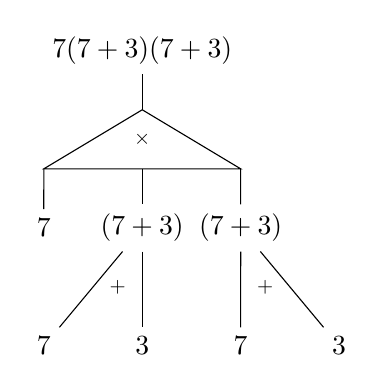
\begin{tikzpicture}[xscale=1.25,yscale=0.75]
        \node (t) at (0,1) {$7(7+3)(7+3)$};
        \node (a) at (-1,-2) {$7$};
        \node (b) at (0,-2) {$(7+3)$}; 
        \node (c) at (1,-2) {$(7+3)$};
        \node (e) at (-1,-4) {$7$};
        \node (f) at ( 0,-4) {$3$};
        \node (g) at ( 1,-4) {$7$};
        \node (h) at ( 2,-4) {$3$};

        \draw (0,0) -- (-1,-1) -- (1,-1) -- cycle;

        \node[scale=0.75] at (0,-0.5) {$\times$};
        \node[scale=0.75] at (-0.25,-3) {$+$};
        \node[scale=0.75] at ( 1.25,-3) {$+$};

        \draw[-] (t) -- (0,0);
        \draw[-] (-1,-1) -- (a);
        \draw[-] (0,-1) -- (b);
        \draw[-] (1,-1) -- (c);
        \draw[-] (b) -- (e);
        \draw[-] (b) -- (f);
        \draw[-] (c) -- (g);
        \draw[-] (c) -- (h);
    \end{tikzpicture}    
\end{center}    
In particular we have not even expressed this as a pair of products 
we have asked instead for a function that takes products of three 
numbers at once.  The ambiguity of how we might achieve this is hidden in the 
triangle \emph{operad} labeled $\times$.
\end{remark}

\section{Formulas: The Free algebra}

There is an evolving pattern in how we described a grammar first for strings, 
then Boolean algebras, and now polynomials.  They each rely on some 
constants set aside at the start.  They also allow for a separate sort for
variables.  Add a final sort for operators and we can describe all the formulas 
we expect in such an algebra.

Now let us notice the pattern.  Our Boolean algebra and our polynomial algebra each 
came in certain form.
\begin{Gcode}[]
    <Formulas<Var>> ::= <Var>
            | <Constants>
            | <Operators>
\end{Gcode}
In fact we can separate operators into order based on how many terms they depend on,
the \emph{valence}, equivalently the degree of the eventual parse tree should that 
production be found in a string.  Letting constants qualify as null-valent operators 
then we have the structure:
\begin{Gcode}[]
    <Formulas<Var>> ::= <Var>
            | <nullvalent operators>
            | <univalent operators>
            | <bivalent operators>
            ...
\end{Gcode}
Or we may abstract in the coarser direction and observe simply the structure operators:
\begin{Gcode}[]
    <Formulas<Var>> ::= <Var>
                      | <Operators>
\end{Gcode}

\begin{definition}
    A \emph{signature} $\sigma$ of an algebra is an (unambiguous) context-free grammar 
    whose production rules are called \emph{operator signatures}.

    A formula with signature $\sigma$ with variables in an alphabet $X$
    is a string accepted by the grammar:
    \begin{Gcode}[]
        <$F_{\sigma}$<X>> ::= <X> | <$\sigma$>
    \end{Gcode}
\end{definition}


\begin{definition}
    A \emph{free algebra} $F_{\sigma}\langle X\rangle$ 
    of a fixed signature $\sigma$ and variables $X$
    is the language accepted 
    \begin{Gcode}[]
        <$F_{\sigma}$<X>> ::= <X> | <$\sigma$>
    \end{Gcode}
    That is, the well-formed formulas with variables $X$.
\end{definition}
\section*{Exercises}

\begin{enumerate}
    \item Write down a grammar to accept natural numbers as digits.  Remember $07$ is not proper substitute for $7$.
    \item Make a grammar to describe rational numbers.
    \item Make a grammar to describe decimal numbers, call this \code{<Reals>}.  
    \item Augment your \code{<Reals>} to include constants for $\pi$ and $e$.
    \item Give a full grammar for real polynomials including conventional short-hand 
    such as $x$ for $x^1$ and $ax$ instead of $(a)(x)$.
    
    \item Suppose that we want to able to add a tally mark to either the left (L) or right (R).
    Define a grammar that allows.  Explain why this is not a model for the natural numbers.
        
    \item Turn the following function into code in both functional and procedural dialects.
    \begin{align*}
        f(n) & = \begin{cases}
                    0 & n=0\\
                    S0 & n=S(k)
        \end{cases}
         =\begin{cases} 0 & n=0 \\ 1 & \text{else}\end{cases}.
    \end{align*}
    
    \item Define multiplication of natural numbers from the Peano grammar given.
\end{enumerate}


% \cleardoublepage